\chapter{Introduction to Common Intermediate Language}
\section{CIL Fundamentals}
The way CIL code get written are arranged by stack. So assume we have the following code in C\#:
\lstinputlisting[style=customcs]{codes/Chap7/Chap7Snippet1.cs}
That code would be compiled as follow:
\lstinputlisting[style=customcs]{codes/Chap7/Chap7Snippet2.cs}

There are few things happening here:
The shorthand CIL opcode, "ldarg.0", loads the first parameter, int a, to the stack. "ldarg.0" is a short hand opcode that you do not have to specify an argument for which parameter to load after opcode, so it save space and serves as a shortcut for runtime to infers what operation to build for that opcode.

Then "ldarg.1" do a similar operation to the above, but load the second parameter onto the stack. The "add" operation requires no arguments, but it pop off 2 items off the stack, so in "add" opcode point of view, when it pop the stack, it would see "ldarg.1" first and then "ldarg.0" second, this is something to keep in mind if you were to plan on writing a new runtime. The "add" opcode will arrange the items that were popped off the stack and do an addition operation from there (it uses the left-hand value type for addition) and then push the result of the addition to the stack.

Now that we have one remaining item in our stack, the "ret" opcode will pop the item off the stack and return that value for function return value.
\newpage
In an effort to help you actually be able to visualize and understand how this works:

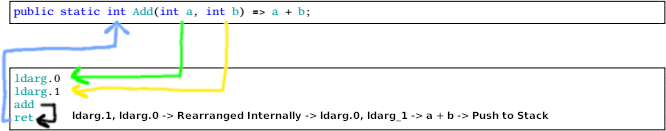
\includegraphics[width=\textwidth]{ChapSevenVisual}

There is another thing to note about CIL, the local variables have to be declared and defined before body of CIL code can be written.

\section{Special Note about the Stack}
\textit{Note: This is a simple warning for those who use Stack in .Net Framework.}

Stack is a Last In First Out, LIFO, so basically the last item you \textbf{push} to the stack is going to be the first item you get when you \textbf{pop} the stack. In .Net Framework, when you attempt to use the IEnumerator of Stack<T>, it will use the pop order in the way you read, so if you for an example have the following code:

\lstinputlisting[style=customcs]{codes/Chap7/Chap7Snippet3.cs}

There is a few things happening here, the stack would be reversed when the following code get called:

\lstinputlisting[style=customcs]{codes/Chap7/Chap7Snippet5.cs}

The stack already get reversed, because remember, the IEnumerator in Stack<T> is read by pop order, so when you pop and push to alternative stack, it rearrange the items like so:

ABC -> CBA -> ABC

To avoid this, you simply just have the following code instead of having to do any additional operations:

\lstinputlisting[style=customcs]{codes/Chap7/Chap7Snippet4.cs}

\newpage
\section{Static vs Class Member Methods}
In CIL, there is a special rule to follow for Static Method and Class Member Methods, static load the first parameter using "ldarg.0", but in class member method, it would load first parameter using "ldarg.1", not "ldarg.0". Because in class member method, "this" is a hidden parameter that get loaded when "ldarg.0" get called and this is a part of a calling convention in C\#.

\lstinputlisting[style=customcs]{codes/Chap7/Chap7Snippet6.cs}

\newpage

\section{Introducing the Dynamic Method}
For creating and building CIL code at runtime, there are three common approaches to this:
\begin{enumerate}
\item DynamicMethod
\item MethodBuilder
\item Assembly Loading via Reflection
\end{enumerate}

Although there are technically infinite amount of approaches you can do it which can involve breaking the Runtime, using unsafe code, or creating your own compiler that works similarly to Roslyn compiler infrastructure.

\subsection{Dynamic Method Approach}
A dynamic method can be defined by using the constructor and specifying the name of method, the return type and parameter types.

\lstinputlisting[style=customcs]{codes/Chap7/Chap7Snippet7.cs}

The DynamicMethod is a shortcut that uses pre-defined dynamic assembly and nest the delegate as a Global Method which are methods that are defined globally in assembly without needing to reside in a type.

\newpage

\subsection{Method Builder Approach}
A dynamic method can also be defined by first defining a dynamic assembly, module, and a type under it. It offers an additional amount of control how you emit your code by managing where code should resides in. You can also optionally choose to define method as a global method similarly to Dynamic Method above.

\lstinputlisting[style=customcs]{codes/Chap7/Chap7Snippet8.cs}

There are a number of objects that have to be defined and it chain all the way to the top starting with an Assembly, the module, the type to contains our method and finally the method itself. There are few things to explain on MethodAttributes and TypeAttributes here, similarly to C\#, we have to define our methods and types with visibility modifiers and constraints. For a static class, it's usually defined by a combination of TypeAttributes.Class, TypeAttributes.Sealed, and TypeAttributes.Abstract which essentially informs the CLR that it's a type that can't be instanced since it's sealed which cannot be inherited from and that it's an abstract which means it doesn't have a constructor to begin with. It's in all essence, a static class.

\newpage

\subsection{Assembly Loading via Reflection}
In an exceptional cases, you may have a custom compiler that generates a custom assembly library, this is one form of an unorthodox dynamic code emitting at runtime. One such form can be done through Roslyn compiler infrastructure which allows you to compile C\# snippet into a .Net assembly which can then be loaded dynamically.

\lstinputlisting[style=customcs]{codes/Chap7/Chap7Snippet9.cs}

The above constructs a .Net Assembly by leveraging Roslyn, we starts by defining our System library for .Net Assembly to reference on (so Runtime objects can be defined.) Then we have a simple snippet for C\# code to compile by using CSharpSyntaxTree that simply deconstruct our parsed text into SyntaxTree which we can then pass to CSharpCompilation object to emit the compiled code as a new .Net Assembly. Through reflection, we can then load the newly created .Net Assembly and select our Math type and it's method to call Add function.

\newpage

\section{Branches in CIL}

The CIL arrangement for branching works by specifying which "line" of CIL code to jump to or if talking about marked labels in System.Reflection.Emits, then it would jump to specified marked label. We can begin a demonstration of this by dynamically emitting a simple for loop code:

In a normal C\# snippet for a For-Loop, it can be written like this:

\lstinputlisting[style=customcs]{codes/Chap7/Chap7Snippet12.cs}

Now the same representation for above in CIL can be written as this:

\lstinputlisting[style=customcs]{codes/Chap7/Chap7Snippet10.cs}

And to help visualize what's happening here, the snippet below is a C\# equivalence to the CIL representation above:

\lstinputlisting[style=customcs]{codes/Chap7/Chap7Snippet11.cs}

\newpage

There are a number of things happening in the snippet above and it can be broken down into these steps:

\begin{enumerate}
\item Define our local variable, an index
\item Define our marks, a body and a condition
\item Emit br to condition label since for-loop requires condition to be evaluated first
\item Mark the label body at this point
\item Emit invocation for Console.WriteLine with our index variable for argument
\item Increment the index variable by 1 at the end of body stub
\item Mark label condition at this point
\item Emit Ldloc\_0 (our local variable is defined first) and Ldc\_I4 with an argument of 10
\item Emit the CLT (Compare Less Than) comparison opcode to compare index to 10
\item Emit brtrue with body label as an argument, return to body if above condition return true
\end{enumerate}

\section{OpCodes references}
You will often find a huge variety of OpCodes, but you might be asking how would you find out what each OpCode do.

The common method is to use documentation which is well maintained: \href{https://docs.microsoft.com/en-us/dotnet/api/system.reflection.emit.opcodes}{https:\/\/docs.microsoft.com\/en-us\/dotnet\/api\/system.reflection.emit.opcodes}

 For each OpCode page, it would list the description, the stack transitional behavior and the relevant overload for emit. To understand the stack transition behavior, hypothetically, you're reading on Add opcode, it would list the following Stack Transitional Behavior:

\begin{enumerate}
\item value1 is pushed onto the stack. 
\item value2 is pushed onto the stack. 
\item value2 and value1 are popped from the stack; value1 is added to value2. 
\item The result is pushed onto the stack. 
\end{enumerate}

It should be fairly clear what's happening, but if you attempt to read the same for subtraction opcode, then it would be important to know which value is a left hand value and which is the right hand value. The third item will explains that "value1 is added to value2" and that clearly define which value is left hand and vice versa.

\subsection{Note about Strict Emit Utility}
\href{https://github.com/Firwood-Software/StrictEmit}{Strict Emit} is also a free library provided by Firwood Organization  that offers a large set of extension methods for ILGenerator to further simplify and document your code.

\newpage

\section{Try Catch Finally Stubs}
The try/catch/finally in CIL are particularly similar to C\# counterpart, but there are some key differences:

\begin{enumerate}
\item There is no "Try" clause in CIL emitting IE in System.Reflection.Emits, it's simply Begin/End Exception Block that enclose entire Try/Catch/Finally clauses. Although in actual CIL Output, the .try clauses will be emitted.
\item Nested Exception Handling will have Catch/Fault blocks filter exception based on the current nested exception block.
\end{enumerate}

In the following example, the code will attempts to create a scenario that the Overflow Exception by attempting to increment an integer that have been signed to maximum value possible.

\lstinputlisting[style=customcs]{codes/Chap7/Chap7Snippet13.cs}

The way BeginCatchBlock works is that when the specified exception were caught, it would have exception available on the stack that you can pop or store into local variable, in this example, it get stored into the second local variable and then it get loaded to print to standard output.

BeginFinallyBlock except a stub of code that will happen in either cases when exception is thrown and when code run successfully without exception.

\newpage

\subsection{Fault Exception Handling}
The fault clause is specific to CIL and isn't a valid keyword for C\#, and it is similar to finally clause, except it's whenever exception get thrown, it doesn't get executed when program exit try clause normally.

To demonstrate the fault handler:

\lstinputlisting[style=customcs]{codes/Chap7/Chap7Snippet14.cs}

\textit{Note: This code may not works on CoreCLR, but it does reflect the expected behavior on Mono Runtime}

To summarize, the Fault Handler is essentially a catch all clause that only run whenever an exception get thrown.

\subsection{Filter Handling}
